\documentclass[border=10pt]{standalone}
\usepackage[svgnames]{xcolor}
\usepackage{amsmath}
\usepackage{pgfplots}
\pgfplotsset{compat=newest}
\usepackage[sfdefault]{FiraSans}
\usepackage{FiraMono}
\renewcommand*\familydefault{\sfdefault}
\begin{document}
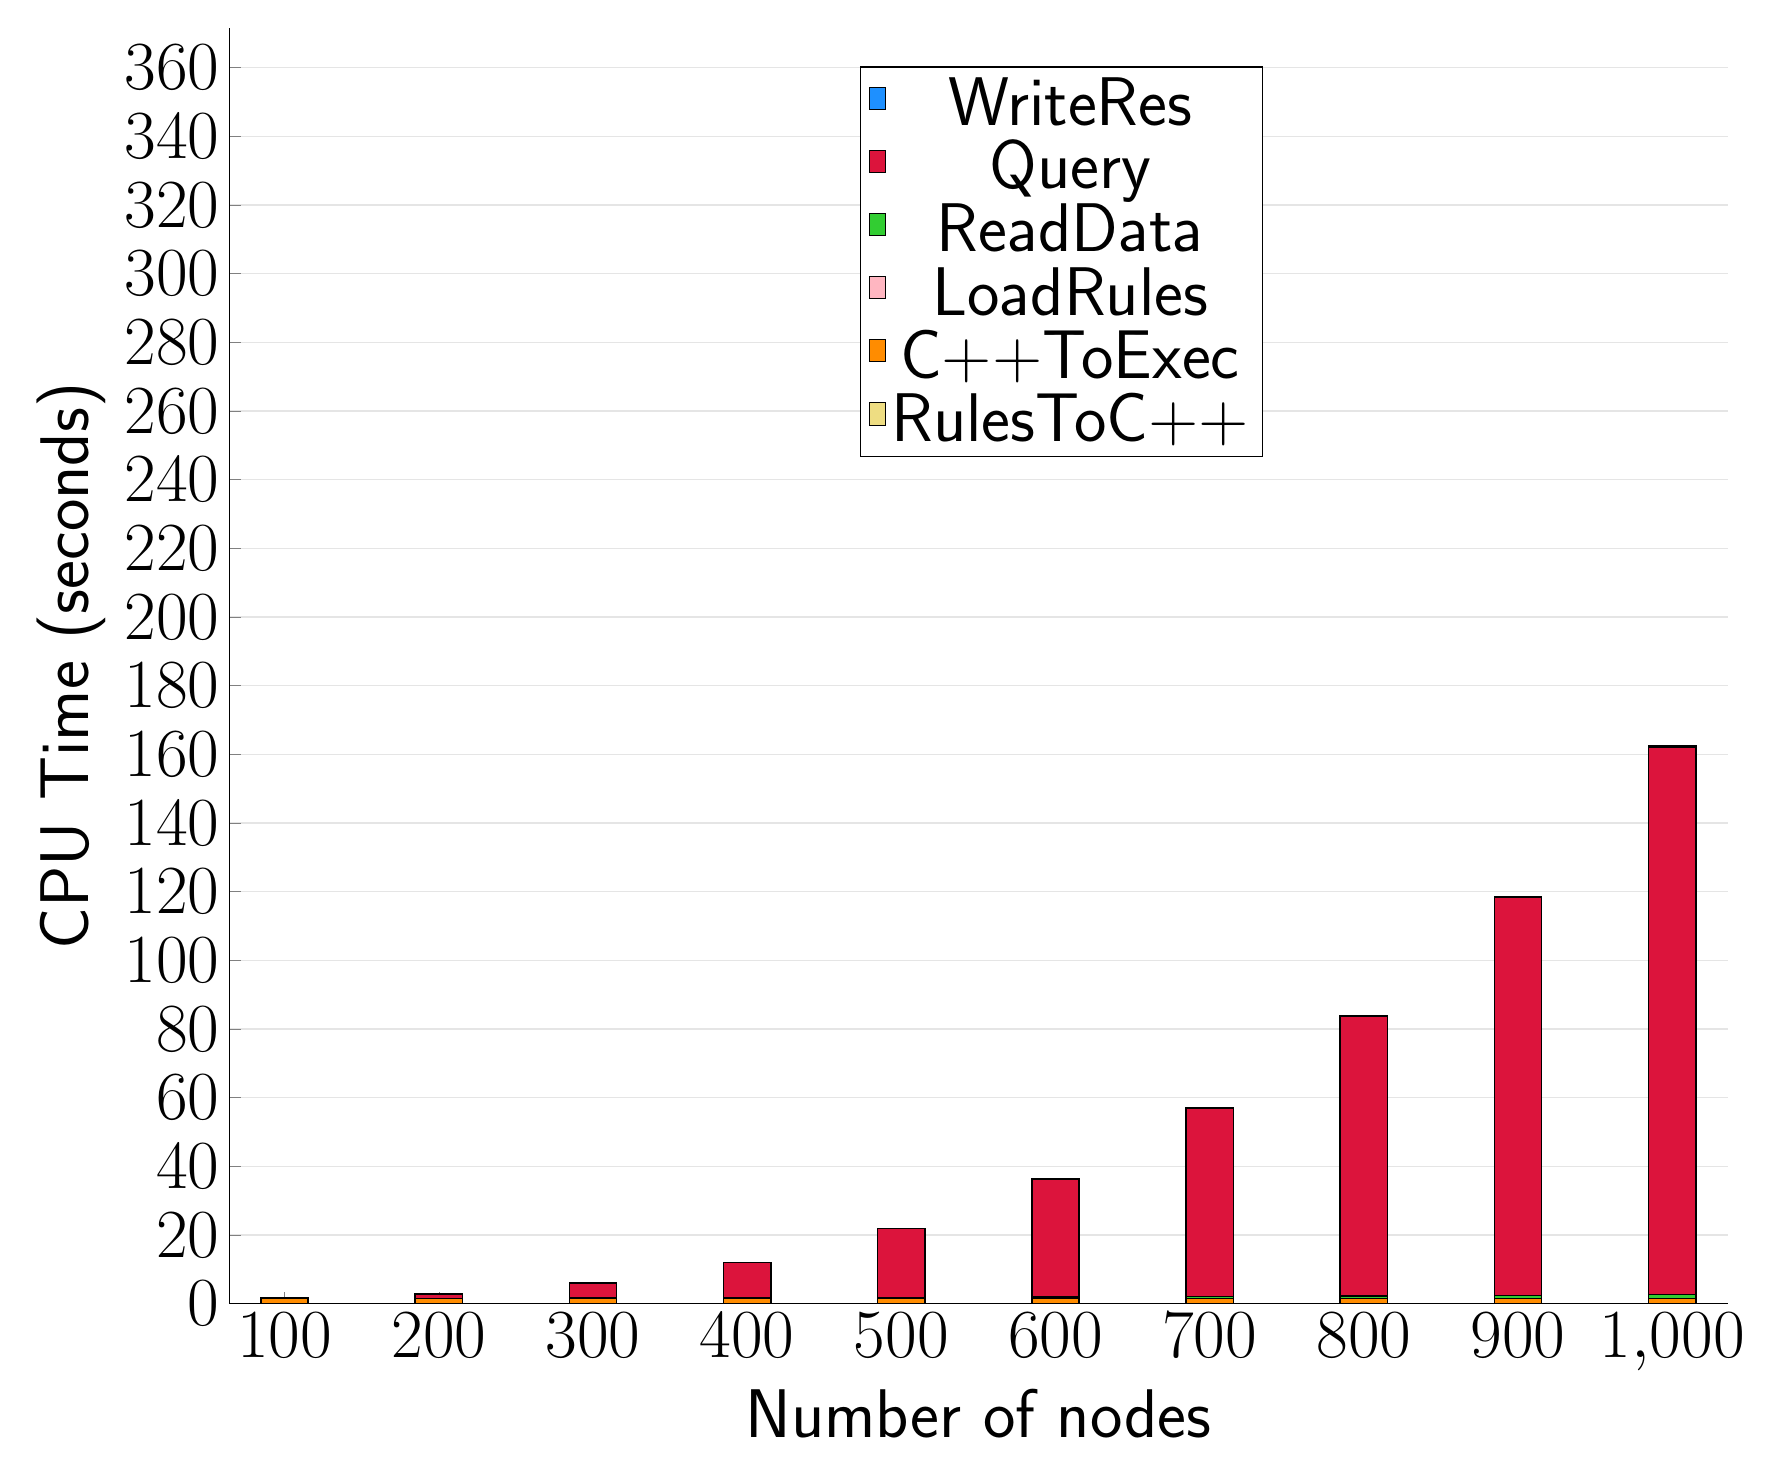
\begin{tikzpicture}
\begin{axis}[
   ybar stacked,
   width=1.7\textwidth,
   bar width=0.6cm,
   ymajorgrids, tick align=inside,
   major grid style={draw=gray!20},
   xtick=data,
   ymin=0, ymax=371.479,
   axis x line*=bottom,
   axis y line*=left,
   enlarge x limits=0.04,
   legend style={
       at={(0.69, 0.97)},
       anchor=north east,
       legend columns=1,
       font=\Huge,
   },
   ylabel={CPU Time (seconds)},
   xlabel={Number of nodes},
   label style={font=\Huge},
   tick label style={font=\Huge},
]
\addlegendimage{fill=DodgerBlue, draw=black, line width=0.2pt}
\addlegendentry{WriteRes}
\addlegendimage{fill=Crimson, draw=black, line width=0.2pt}
\addlegendentry{Query}
\addlegendimage{fill=LimeGreen, draw=black, line width=0.2pt}
\addlegendentry{ReadData}
\addlegendimage{fill=LightPink, draw=black, line width=0.2pt}
\addlegendentry{LoadRules}
\addlegendimage{fill=DarkOrange, draw=black, line width=0.2pt}
\addlegendentry{C++ToExec}
\addlegendimage{fill=LightGoldenrod, draw=black, line width=0.2pt}
\addlegendentry{RulesToC++}
\addplot +[fill=LightGoldenrod, draw=black, line width=0.55pt] coordinates {
(100, 0.008000000000000002)
(200, 0.004000000000000001)
(300, 0.008000000000000002)
(400, 0.0020000000000000005)
(500, 0.0020000000000000005)
(600, 0.0020000000000000005)
(700, 0.0)
(800, 0.0)
(900, 0.0)
(1000, 0.0)
};
\addplot +[fill=DarkOrange, draw=black, line width=0.55pt] coordinates {
(100, 1.472)
(200, 1.482)
(300, 1.482)
(400, 1.4899999999999998)
(500, 1.488)
(600, 1.4760000000000002)
(700, 1.4819999999999998)
(800, 1.482)
(900, 1.474)
(1000, 1.476)
};
\addplot +[fill=LightPink, draw=black, line width=0.55pt] coordinates {
(100, 0.0001718)
(200, 0.0001714)
(300, 0.0001638)
(400, 0.0001738)
(500, 0.00016479999999999997)
(600, 0.00019319999999999998)
(700, 0.000191)
(800, 0.0001898)
(900, 0.000203)
(1000, 0.00019940000000000002)
};
\addplot +[fill=LimeGreen, draw=black, line width=0.55pt] coordinates {
(100, 0.025143200000000004)
(200, 0.0683648)
(300, 0.1247746)
(400, 0.20489039999999997)
(500, 0.30804580000000004)
(600, 0.43432780000000004)
(700, 0.5867352)
(800, 0.757899)
(900, 0.9560248)
(1000, 1.1800599999999999)
};
\addplot +[fill=Crimson, draw=black, line width=0.55pt] coordinates {
(100, 0.1748882)
(200, 1.288402)
(300, 4.312656)
(400, 10.2421)
(500, 20.02474)
(600, 34.37328)
(700, 54.81555999999999)
(800, 81.53943999999998)
(900, 115.973)
(1000, 159.53879999999998)
};
\addplot +[fill=DodgerBlue, draw=black, line width=0.55pt] coordinates {
(100, 0.0023746)
(200, 0.0089314)
(300, 0.019713)
(400, 0.034501)
(500, 0.054256799999999994)
(600, 0.0779796)
(700, 0.10419199999999999)
(800, 0.1352344)
(900, 0.1724408)
(1000, 0.2128844)
};
\end{axis}
\end{tikzpicture}

\end{document}
